\documentclass[journal]{IEEEtran}
\usepackage{blindtext}
\usepackage{graphicx}
\usepackage{listings}
\usepackage[superscript,biblabel]{cite}


\hyphenation{op-tical net-works semi-conduc-tor}

\begin{document}

\title{Cellular Languages}

\author{Breck~Yunits% <-this % stops a space
\thanks{Remember, you can't spell Phony Dumbass without PhD.}% <-this % stops a space
}

\markboth{February~2023 DRAFT}%
{Shell \MakeLowercase{\textit{et al.}}: Bare Demo of IEEEtran.cls for Journals}

\maketitle


\begin{abstract}
%\boldmath
I introduce new terminology for the next generation of human-computer languages.
\end{abstract}

\IEEEpeerreviewmaketitle

\section{Introduction}

A strand of nucleic acids is useless in 99.\overline{9}$\% positions in the universe. But the right strand placed in the right cell changes history. Nucleic acids are nature's language and cells are nature's parsers and compilers. Nature's languages are not only context sensitive, but \textit{context is everything}.

This ubitiquous truth has been lost on programming language designers focused on Context-Free Grammars. In this paper I hope to provide a new way to look at Context Sensitive Languages—as \textbf{Cellular Languages}— and hopefully convince aspiring thinkers to explorer this largely overlooked field of research which I predict will yield significantly simpler and more efficient languages than our current crop.

\section{Cellular Languages}

Cellular Languages are languages recursively composed of other Cellular Languages where certain languages are active or inactive in different cells of a program. A program consists of multiple cells, and each cell may have different languages active.

The rules and language may change entirely depending upon where in the program one is.

\begin{figure}[ht!]
\centering
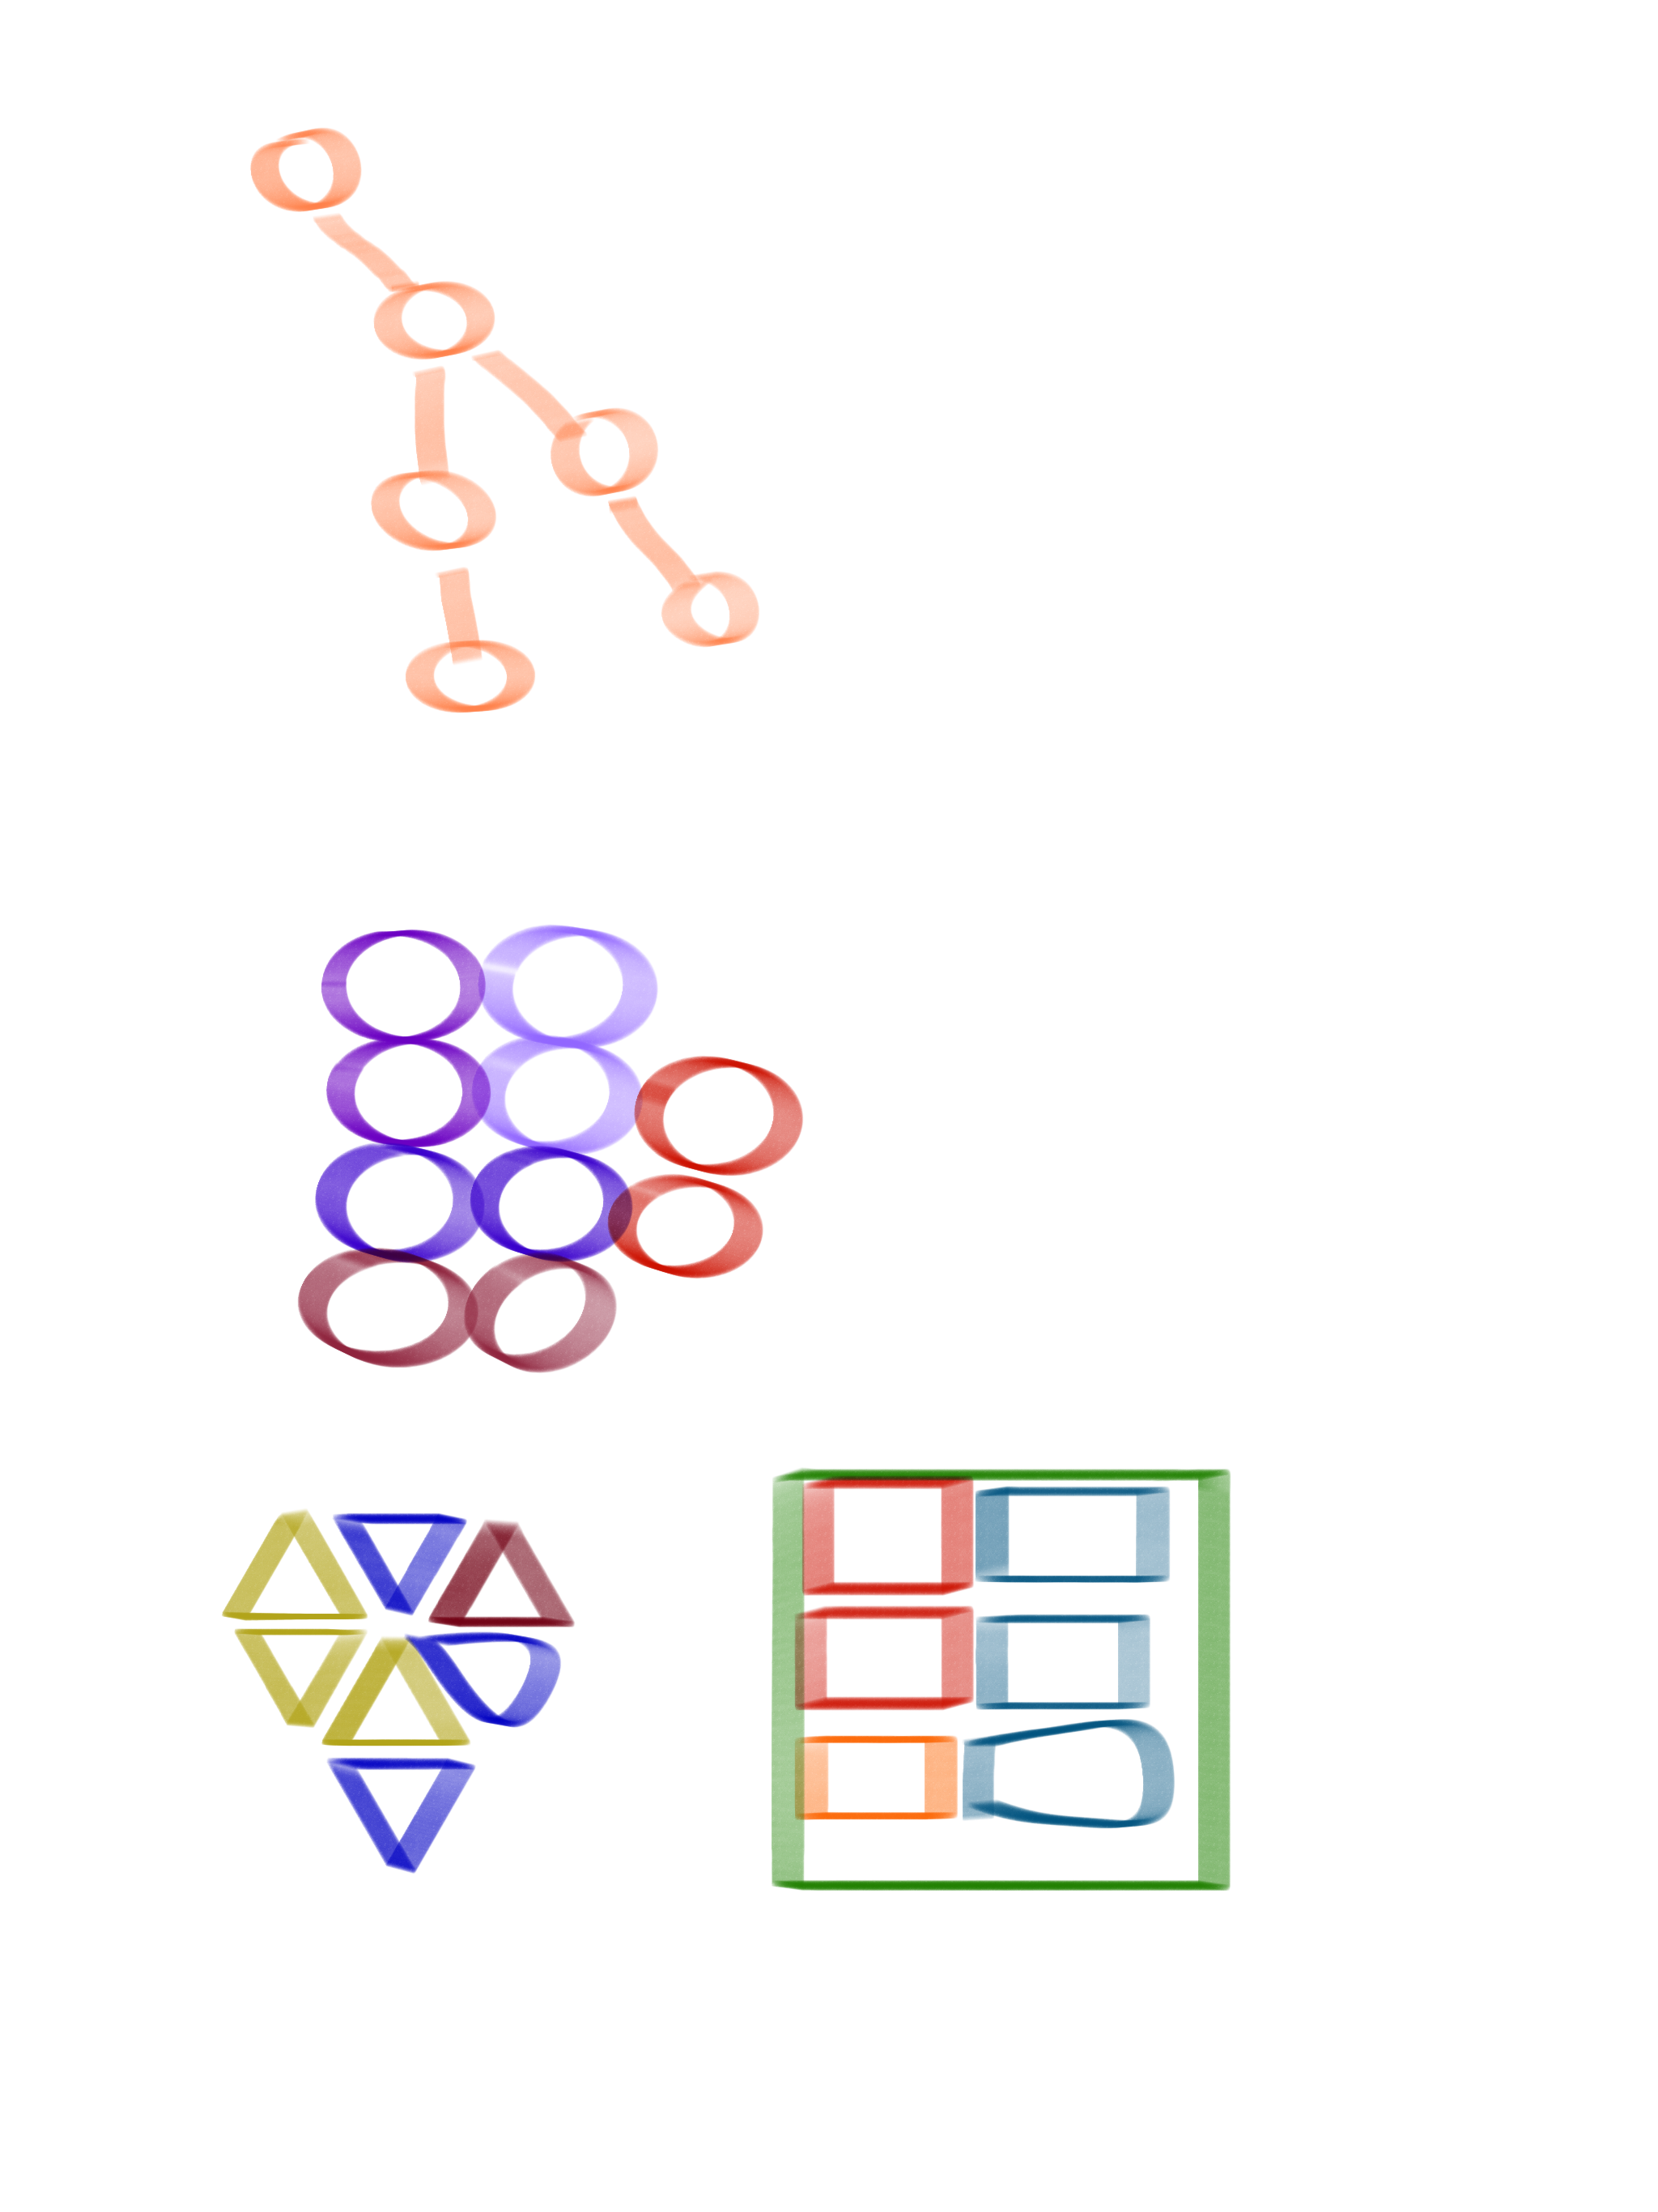
\includegraphics[width=90mm]{sketch.png}
\caption{In the top picture the language remains constant for the whole program. In the bottom pictures different Cellular Languages are active in different cells of the program. Programs are similar to multi-cellular organisms.}
\end{figure}

\section{Examples}

\section{Grammar Languages for Cellular Languages}

\section{Conclusion and Future Work}

\end{document}
